%%%%%%%%%%%%%%%%%%%% author.tex %%%%%%%%%%%%%%%%%%%%%%%%%%%%%%%%%%%
%
% sample root file for your "contribution" to a contributed volume
%
% Use this file as a template for your own input.
%
%%%%%%%%%%%%%%%% Springer %%%%%%%%%%%%%%%%%%%%%%%%%%%%%%%%%%


% RECOMMENDED %%%%%%%%%%%%%%%%%%%%%%%%%%%%%%%%%%%%%%%%%%%%%%%%%%%
\documentclass[graybox]{svmult}

% choose options for [] as required from the list
% in the Reference Guide
\usepackage{amssymb}
\usepackage{graphicx}
\usepackage{caption}
\usepackage{subcaption}
\usepackage[colorlinks,linkcolor=blue]{hyperref}
\usepackage{todonotes}
\usepackage{type1cm}        % activate if the above 3 fonts are
                            % not available on your system
%
\usepackage{makeidx}         % allows index generation
\usepackage{graphicx}        % standard LaTeX graphics tool
                             % when including figure files
\usepackage{multicol}        % used for the two-column index
\usepackage[bottom]{footmisc}% places footnotes at page bottom


\usepackage{newtxtext}       % 
\usepackage[varvw]{newtxmath}       % selects Times Roman as basic font
\usepackage{wrapfig}

% see the list of further useful packages
% in the Reference Guide

\makeindex             % used for the subject index
                       % please use the style svind.ist with
                       % your makeindex program

%%%%%%%%%%%%%%%%%%%%%%%%%%%%%%%%%%%%%%%%%%%%%%%%%%%%%%%%%%%%%%%%%%%%%%%%%%%%%%%%%%%%%%%%%

\begin{document}

 \title*{\textbf{TransportIDE} -- An integrated transportation system design and simulation environment}
\titlerunning{TransportIDE} 
%\author{Anonymous Author and Anonymous Author}
\author{Dominik Ascher and Georg Hackenberg}
% Use \authorrunning{Short Title} for an abbreviated version of
% your contribution title if the original one is too long
\institute{Dominik Ascher \at Distributed Artificial Intelligence Laboratory, Faculty of Electrical Engineering and Computer Science, Technical University of Berlin, 10587 Berlin, Germany, \email{ascher@tu-berlin.de}
	\and Georg Hackenberg \at School of Engineering, University of Applied Sciences Upper Austria, 4600 Wels, Austria,
	\email{georg.hackenberg@fh-wels.at}}
%\institute{Anonymous Author \at Space reserved for author affiliation
%\and Anonymous Author \at Space reserved for author affiliation
%}
%
% Use the package "url.sty" to avoid
% problems with special characters
% used in your e-mail or web address
%
\maketitle
%\abstract*{AA.}
\abstract{%As transportation systems have to become more intelligent, efficient and, ultimately, sustainable, the complexity of designing these systems has increased fundamentally.
	%This observation holds true both for person transport and for good transport, on public infrastructure and on private infrastructure.
	%Designing efficient transportation systems is a difficult undertaking due to the vast size of the solution space and the emergent dynamics of the system components, which have to be considered. %Therefore, transportation system engineers need appropriate tools and methods to wholistically explore the design space and test solutions quickly and reliably. In this paper, we propose a simulation-based environment using discrete event simulation (DES) for transportation system design, which is based on a formal system theory. 
	The interconnection between intelligent transportation systems (ITS) and services poses fundamental challenges with respect to establishing most efficient structures, infrastructures, as well as intelligent and integrated control strategies addressing new transportation paradigms such as autonomous vehicles, demand-responsive transport as well as the transportation electrification. Systematic methods for efficiently modeling, simulating and evaluating these systems are required, which are able to address aforementioned challenges.
	For this, we present a formalization of essential static properties, dynamic state functions, as well as events concisely describing transportation system design space in the scope of emerging transportation paradigms. Our proposed formalization allows for reduction of simulation complexity by focusing on relevant events impacting the design problem at hand only, while omitting unimportant details negatively impacting simulation performance, thereby reducing both modeling as well as simulation effort. In addition, the provided formalization of system theory and discrete events serves as an interface for deriving well-defined system structure as well as efficient control strategies. 
}
	%Furthermore, we demonstrate possible applications such as comparison of different infrastructure and control algorithm designs.}
\vspace{-2mm}
  \section{Introduction}
\label{sec:intro}
Meeting sustainability goals and reducing carbon emissions \cite{sachs2019six} is a driving factor of the transformation of transportation systems towards their more efficient operation. In this, new and connected transportation paradigms such as autonomous vehicles, demand-responsive transport \cite{brake_demand_2004} as well as the transportation electrification \cite{pereirinha2018main} provide fundamental and, more significantly, conjoined drivers towards intelligent transportation systems (ITS) and services.
However, the interconnection between intelligent transportation systems (ITS) and services poses fundamental challenges, in particular with respect to establishing most efficient structures, infrastructures, as well as intelligent and integrated control strategies. Quality assurance of these systems and services is a critical challenge as constituting systems and services form integrated system-of-systems with heterogenous system requirements, goals, constraints and stakeholders, which need to be systematically adressed by integrated system design and control strategies. Therefore, systematic development methods for these challenges as well as these emerging domain paradigms are required.

%Demand-responsive transport \cite{brake_demand_2004} as well as the transportation electrification \cite{pereirinha2018main} represent two current key emerging domain paradigms in transportation systems. The former describes covering transportation demands arising from passengers or freights demanding transport from a given source origin to a target destination using a supply of vehicles, which are dispatched with respect to covering a set of objectives such as shortest-traveling time, energy-efficient operation, or their balanced distribution on the transport infrastructure. Then, transportation electrification describes the increasing penetration of electric vehicles in the transportation system, which pose new challenges over traditional, i.e. combustion engine, vehicles such as possibily more limited ranges, which have to considered in accordance to or constrained by a given charging infrastructure. 
\vspace{-2mm}

\subsection{Related Work}
%In the following, we provide an overview of the state of the art and related work on transportation system modeling and simulation.

%In terms of simulation frameworks tailored to the transport domain, traffic simulators such as PTV Vissim \cite{fellendorf_vissim_1994}, MATSim \cite{w_axhausen_multi-agent_2016}, and SUMO \cite{krajzewicz2010traffic}, \cite{lopez_microscopic_2018} are widely established on a domain-wide level. SUMO represents a microscopic traffic simulation employing various microscopic models such as a car-following model \cite{krauss1998microscopic} determining driving dynamics of vehicles based on the positions and velocities of neighboring vehicles, a lane-changing model \cite{erdmann2015sumo}, which determines lane choices on multi-lane roads and required speed adjustments, as well as a intersection model \cite{krajzewicz2013road}, which determines behavior of vehicles at intersections. In addition, mesoscopic models \cite{eissfeldt2004vehicle} have been adopted by SUMO in selective extensions such as MESO.

To describe, evaluate and compare integrated transportation system design options systematically, we previously introduced an approach for modeling integrated intelligent transportation system properties which addresses scenarios such as vehicle-to-grid (V2G) interactions on both transportation and power systems \cite{Ascher2015}, \cite{Ascher2016} and electrified autonomous mobility-on-demand systems \cite{Ascher2017}. As simulation complexity increases with the number and dimensionality of states and actions of the modeled systems as well as decreasing sizes of fixed time discretization steps, our approach was limited to microscopic design problems with impeded simulation accuracy, where for instance detection of collision events between traffic participants was dependant on sufficiently small time discretization and sampling steps.

Discrete-event simulation (DES) represents an approach which significantly reduces simulation complexity by limiting number and dimensionality of actions, while abstracting from discrete-time resolutions. In recent years, DES has seen increased research attention in both transportation \cite{clemente2013discrete, fanti2017fleet} and power \cite{lebeau2013implementing, ferro2019predictive, lopez2021modeling} domains. For instance, Clemente et al. \cite{clemente2013discrete} propose a discrete event simulation approach in the context of car sharing, where a fleet of vehicles is shared and utilized, i.e. driven and parked, by customers. However, compared to our scope, they do not model the interactions arising from autonomous electric vehicles in the scope of mobility-on-demand systems, such as demand responsive transport and interactions with a charging infrastructure. Lopez et al. \cite{lopez2021modeling} model electric vehicle charging and derived hourly and weekly electricity demands using a DES-based model. They focus on modeling at home charging behavior of electric vehicles of private users, compared to our scope, which instead focuses on modeling both transportation and charging demands of fleets of shared autonomous electric vehicles. Finally, Li et al. \cite{li2021simulation} model electric carsharing systems using a discrete-event simulation based approach. For this, they consider infrastructures such as charging stations and links, as well as electric vehicles and transport demands in their proposed model.

\subsection{Problem Statement}

Current approaches for modeling, simulating and evaluating transportation system designs are not able to holistically address integrated system challenges. On the one hand side, transportation infrastructures and control algorithms need to be holistically evaluated, based on the heterogenous systems they are composed of and the heterogenous requirements they have to adhere to. On the other hand side, simulation complexity of integrated systems rises according to model complexity, such as employed discretization of time resolution, as well as number and dimensionality of system states and actions. While the approach of discrete event simulation is able to address latter problems, current modeling approaches for system design do not offer appropriate domain abstractions in terms of their provided structural and behavioral modeling capabilities to describe these systems on a required level of detail. In addition, the approaches do not offer support for evaluating heterogenous application scenarios in terms of their configuration space for new transportation paradigms. Therefore, we consider it important to assess the following research question: Which set of essential system properties, dynamic state functions as well as events are necessary and relevant for describing integrated system problems in the context of emerging transportation paradigms such as autonomous vehicles, demand-responsive transport and the transportation electrification?

\vspace{-2mm}

%\subsection{Research questions}
%With respect to these challenges, we pose the following research questions:
%\begin{itemize}
%	\item RQ1: How can we support the design and test of transportation infrastructures and control algorithms better?
%	\item RQ2: Which modeling and simulation technique represents an appropriate abstraction for the domain?
%	%\item RQ3: Which software architecture is appropriate for an integrated design and test environment?
%	\item RQ3: Which application scenarios should be supported on top of this environment?
%	\item RQ4: Which events to describe for the specific system, and of those, which events are relevant?
%\end{itemize}
%\vspace{-2mm}

\subsection{Contribution}
% Previous approach - Complexity Reduction of simulation using DES, Formalization of system concepts using notation/foundation 
%To answer the above questions, we apply and combine two research methodologies.
%First we conduct a literature review to understand the state of the art in transportation system design and test.
%Second we use iterative and incremental software development with regular feedback from stakeholders to develop our a new dedicated approach.
%To address these challenges and the above research questions, subsequently, we introduce a systematic and iterative approach for transportation system design.

%To describe, evaluate and compare integrated transportation system design options systematically, we previously introduced an approach for modeling integrated intelligent transportation system properties using a formal foundation. However, due to the inherent complexity in defining large-scale problems and evaluating them using simulation, our approach was only applicable to limited scale, i.e. microscopic design problems, and allowed fixed simulation resolution only, where for instance detection of collisions between traffic participants, was dependant on discrete-time resolution.  

%Key Question: Formalization of events, minimum set of states, proposal
%To address these challenges and the above research questions, in this work, we improve upon our previous approach by employing Discrete Event Simulation (DES), which helps reduce simulation complexity significantly, thereby allowing one to now model and evaluate microscopic to macroscopic design problems using our proposed design abstraction. 

To address this situation, in this work, we provide a description and formalization of a concise and essential set of static system properties, dynamic state functions as well as discrete events, which help reduce simulation complexity significantly. 
%allowing one to model and derive control strategies for microscopic to macroscopic transportation system design problems.
This is achieved by focusing on relevant events impacting the design problem at hand only, thereby reducing modeling effort and omitting unimportant details negatively impacting simulation performance, while providing a well-defined notation and interface for deriving sound system design structure and efficient control strategies. In summary, we provide the following contributions:

In Section~\ref{sec:theory} we provide a formalization of the underlying system theory of our approach, which focuses on definition of a concise and essential set of static properties and dynamic states for establishing models of transportation systems in the context of autonomous vehicles, demand responsive transport and the transportation electrification.

In Section~\ref{sec:events}, based on introduced system theory, we provide a formalization of discrete events for determining decisions that must be considered for high-performance state computation, where event-based formalization supports abstraction and complexity reduction of system simulation, and can be utilized for deriving well-defined and efficient control strategies. 

%In Section ~\ref{sec:related}, we investigate related work, and compare our approach.
%Afterwards, we explain our software architecture in Section~\ref{sec:arch}.
%Thereafter, we demonstrate three software applications in Section~\ref{sec:app}.
Finally, in Section~\ref{sec:con}, we conclude with a short discussion of our approach as well as its application for deriving system designs and control strategies, and provide an outlook on future work.
\vspace{-2mm}

\section{System theory}
% Briefly explain system theory of existing work
\label{sec:theory}
In the following, we explain the underlying system theory, which is based on our approach for integrated transportation system design, for which we refer to previous work~\cite{Ascher2014,Ascher2015,Ascher2016,Ascher2017}. We extend and improve upon this approach in this work, where the system theory presented in this work is intended to capture a concise and an essential set of properties and dynamic states for establishing sound models and control strategies for transportation systems. These properties and dynamic states serve as a foundation for further abstraction and reduction of system simulation complexity using discrete events, for which we refer to Section \ref{sec:events}.
%In Section~\ref{sec:concepts} we introduce basic definitions and concepts, which can be used for transportation system design such as properties, states as well as simple and complex functional relations. 
%Then, in Section~\ref{sec:transitions} we show more complex functional relations over the previous concepts, their properties, and their states.
%Finally, in Section~\ref{sec:events} we describe the events and decisions that must be considered for high-performance state computation using discrete event simulation.


%\subsection{Basic definitions}
%\label{sec:concepts}
%In this subsection, we establish basic definitions for concepts, properties, states and simple functional relations in subsection \ref{sec:simple} and then, secondly, complex functional relations in \ref{sec:complex}.

%\subsubsection{Concepts, properties, states, and simple functional relations}
%\label{sec:simple}

\begin{figure*}[t] 
	\centering
	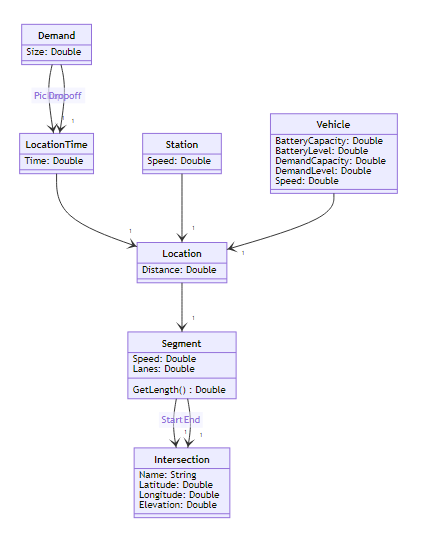
\includegraphics[scale=0.30]{../../diagrams/model/classes-v0.png}
	\caption{Concepts in UML class diagram notation.}
	\label{fig:concepts}
\end{figure*}
For system theory, Figure~\ref{fig:concepts} provides an overview of the model concepts, their properties, and their states.
Here, we use intersections $i \in I$, segments $s \in S$ as well as locations $l \in L$ for describing properties about the transportation infrastructure.
Then, based on the transportation infrastructure, we use charging stations $cs \in CS$ for describing the provided charging infrastructure.
In addition, we describe transportation demands $d \in D$ on the transportation infrastructure. 
Finally, we use vehicles $v \in V$ for describing transportation supply and capacities.
In the following, we describe each concept in more detail including their static (i.e.\ time-independent) properties as well as their dynamic (i.e.\ time-dependent) state functions typically sampled during computer simulations. We describe intersections, segments and locations in Section \ref{sec:intersections-segments}, and charging stations, demands as well as vehicles in Section \ref{sec:chargingstations-demands-vehicles}.

\vspace{-2mm}
% TODO Location-Times
\subsection{Intersections, Segments and Locations}
\label{sec:intersections-segments}
In this Section, we subsequenly describe intersections and segments of the transportation infrastructure as well as locations. These concepts are visualized in Figure \ref{fig:intersections-segments}.

% TODO Figure for Location, Location on Segment, Distance on Segment
\begin{figure}
	\begin{subfigure}{.3\textwidth}
		\centering
		
\includegraphics[scale=0.4]{../../concepts/intersection.png}
		\caption{Intersection}
		\label{fig:intersection}
	\end{subfigure}
	\hfill
	\begin{subfigure}{.3\textwidth}
		\centering
		
\includegraphics[scale=0.4]{../../concepts/segment.png}
		\caption{Segment}
		\label{fig:segment}
	\end{subfigure}
	\hfill
		\begin{subfigure}{.3\textwidth}
		\centering
		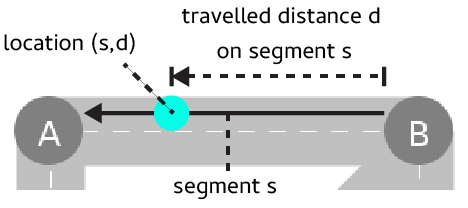
\includegraphics[scale=0.4]{../../concepts/location.png}
		\caption{Location}
		\label{fig:location}
	\end{subfigure}
\hfill
	\caption{Intersections, segments and locations.}
	\label{fig:intersections-segments}	
\end{figure}

\noindent
\textbf{Intersections} (see Figure \ref{fig:intersection})
define the routing points of the transportation infrastructure.
Each intersection must have a coordinate in the corresponding reference coordinate system.
Mathematically, intersections can be described as elements $i \in I$ with the static property function
\begin{itemize}
	\item \textit{coordinate} $P_{I.C}: I \rightarrow \mathbb{R}^3$, i.e. intersection position in Euclidian space.
\end{itemize}
\vspace{2mm}

\noindent
\textbf{Segments} (see Figure \ref{fig:segment})
define the straight roads of the transportation infrastructure.
Each segment must define a source and a target intersection, which represent the start and the end coordinates of the straight road.
The length of the segment can be computed from the coordinates of the source and the target intersection.
Additionally, each segment must define a width and a maximum drive speed.
Mathematically, segments can be described as elements $s = (i_s, i_t) \in I \times I = S$ with source intersection $i_s$, target intersection $i_t$, and static property functions as follows:
\begin{itemize}
	\item \textit{length} $P_{S.L}: S \rightarrow \mathbb{R}_0^+$, i.e. physical extent of segment length. We require that the value equals to the Euclidean distance between the coordinates of the source and the target intersection, i.e.\ $P_{S.L}(i_s, i_t) = |P_{I.C}(i_t) - P_{I.C}(i_s)|$,
	\item \textit{width} $P_{S.W}: S \rightarrow \mathbb{R}^+$, i.e. physical extent of segment width, and
	\item \textit{maximum drive speed} $P_{S.MDS}: S \rightarrow \mathbb{R}^+$, i.e. maximum drive speed permitted for vehicles on the segment.
\end{itemize}
\vspace{-2mm}

%\subsection{Locations and Location-Times}
%\label{sec:locations-locationtimes}	
%In this Section, we subsequently describe locations and location-times on the transportation infrastructure.

\vspace{4mm}
\noindent
\textbf{Locations}
represent an auxiliary concept used to define dedicated positions on the transportation infrastructure.
Each location must define a segment and a travelled distance on that segment.
Mathematically, \textit{locations} can be described as elements $(s, d) \in S \times \mathbb{R}_0^+ = L$ with segment $s$ and distance $d$ such that $d \leq P_{S.L}(s)$.

%\vspace{4mm}
%\noindent
%\textbf{Location-times}
% also represent an auxiliary concept and define dedicated positions on the transportation infrastructure at particular time points.
%Each location-time must define a corresponding location and the desired time point.
%Mathematically, location-times can be described as elements $(l, t) \in L \times \mathbb{T} = LT$ with location $l$ and time point $t$.
%\vspace{-2mm}

\noindent
\subsection{Charging Stations, Demands and Vehicles}
\label{sec:chargingstations-demands-vehicles}	
In this Section, we subsquently describe charging stations, demands as well as vehicles. These concepts are visualized in Figure \ref{fig:chargingstations-demands-vehicles}.
\begin{figure}
	\hfill
	\begin{subfigure}{.3\textwidth}
		\centering
		
\includegraphics[scale=0.25]{../../concepts/charge-station.png}
		\caption{Charging Station}
		\label{fig:charging-station}	
	\end{subfigure}
	\hfill
	\begin{subfigure}{.3\textwidth}
		\centering
		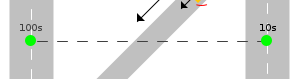
\includegraphics[scale=0.4]{../../concepts/demand.png}
		\caption{Demand}
		\label{fig:demand}
	\end{subfigure}
	\hfill
	\begin{subfigure}{.3\textwidth}
		\centering
		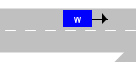
\includegraphics[scale=0.6]{../../concepts/vehicle.png}
		\caption{Vehicle}
		\label{fig:vehicle}	
	\end{subfigure}

	\caption{Charging stations, demands and vehicles.}
	\label{fig:chargingstations-demands-vehicles}	
\end{figure}

\noindent
\textbf{Charging Stations} (see Figure \ref{fig:charging-station})
define the charging infrastructure for vehicles to refill their batteries.
%Each charging station must define a location and a maximum charge speed.
Charging stations $cs \in CS$ define the following static property functions $P_{CS}$:
\begin{itemize}
	\item \textit{location} $P_{CS.L}: CS \rightarrow L$, i.e. a location on the transport infrastructure, and
	\item \textit{maximum charge speed} $P_{CS.MCS}: CS \rightarrow \mathbb{R}^+$, i.e. maximum charge rate imposed by the charging station.
\end{itemize}
%Furthermore, the dynamic state of charging stations comprises the current vehicles and the current charge speed.
%Mathematically, the state of charging stations $cs$ can be described using dynamic state functions with corresponding simple functional relations
In addition, computer simulations typically sample the following dynamic state functions $S_{CS}$ for charging stations $cs \in CS$:
%TODO Empty vehicle description
\begin{itemize}
	\item \textit{current vehicle} $S_{CS.CV}: CS \times \mathbb{T} \rightarrow V \cup \{\perp\}$, i.e. the vehicle currently connected to the charging station, with $\perp$ representing no vehicle connected, and
	\item \textit{current charge speed} $S_{CS.CCS}: CS \times \mathbb{T} \rightarrow \mathbb{R}^+$, i.e. the current charge rate of the charging station. We require that the current charge speed is smaller than or equal to the maximum charge speed of the charging station, i.e.\ $\forall t \in \mathbb{T}: S_{CS.CCS}(cs,t) \leq P_{CS.MCS}(cs)$.
\end{itemize}

\vspace{2mm}
\noindent
\textbf{Demands} (see Figure \ref{fig:demand})
 define the transportation loads that temporarily consume the transportation capacities. Each demand $d \in D$ defines the following static property functions $P_D$:
%Each demand must define a size, a pick-up location, a drop-off location, an earliest pick-up time, and a latest drop-off time.
%Mathematically, demands can be described as elements $d \in D$ with static property functions such that

\begin{itemize}
	\item \textit{size} $P_{D.S}: D \rightarrow \mathbb{R}^+$, i.e. the transport capacity required by the demand,
	\item \textit{appear time} $P_{D.AT}: D \rightarrow \mathbb{T}$, i.e. time of demand appearance in the computer simulation,
	\item \textit{pick-up location and earliest time} $P_{D.PULT}: D \rightarrow L \times \mathbb{T}$ with $P_{D.PULT}(d) = (l_d^{PULT},t_d^{PULT})$, i.e. location and earliest possible time of demand pick-up, and
	\item \textit{drop-off location and latest time} $P_{D.DOLT}: D \rightarrow L \times \mathbb{T}$ with $P_{D.DOLT}(d) = (l_d^{DOLT},t_d^{DOLT})$, i.e. describing location and latest possible time of demand drop-off. We require that the pick-up location is different from the drop-off location, i.e.\ $l_d^{PULT} \neq l_d^{DOLT}$, and the earliest pick-up time is before the latest drop-off time, i.e.\ $t_d^{PULT} < t_d^{DOLT}$.
\end{itemize}
In addition, computer simulations typically sample the following dynamic state functions $S_{D}$ for demands $d \in D$:
% of demands comprises the current vehicle and the current location.
%Mathematically, the state of demands $d$ can be described using dynamic state functions with corresponding simple functional relations such that
\begin{itemize}
	\item \textit{current vehicle} $S_{D.CV}: D \times \mathbb{T} \rightarrow V \cup \{\perp\}$, i.e. the vehicle the demand is currently assigned to, and
	\item \textit{current location} $S_{D.CL}: D \times \mathbb{T} \rightarrow L$, i.e. the current location of the demand on the transport infrastructure.
\end{itemize}

% TODO Note that currently we do not consider a time delay in assignment/loading

\vspace{2mm}
\noindent
\textbf{Vehicles} (see Figure \ref{fig:vehicle})
 define the transportation capacities available on the transportation infrastructure. Each vehicle $v \in V$ must define the following static property functions $P_V$:
 %Each vehicle must define a maximum battery level, a maximum demand level, a maximum drive speed, and a maximum charge speed, an initial location, and an initial battery level.
%Mathematically, vehicles can be described as elements $v \in V$ with static property functions
\begin{itemize}
	\item \textit{length} $P_{V.L}: V \rightarrow \mathbb{R}_0^+$, i.e. the physical extent of vehicle length,
	\item \textit{width} $P_{V.W}: V \rightarrow \mathbb{R}_0^+$ , i.e. the physical extent of vehicle width, 
	\item \textit{maximum battery level} $P_{V.MBL}: V \rightarrow \mathbb{R}^+$, i.e. maximum battery state of charge, 
	\item \textit{maximum demand level} $P_{V.MDL}: V \rightarrow \mathbb{R}^+$, i.e. maximum capacity of the vehicle to transport demands,
	\item \textit{maximum drive speed} $P_{V.MDS}: V \rightarrow \mathbb{R}^+$, i.e. maximum vehicle drive speed, 
	\item \textit{maximum charge speed} $P_{V.MCS}: V \rightarrow \mathbb{R}^+$, i.e. maximum charge rate imposed by the vehicle battery,
	\item \textit{initial location} $P_{V.IL}: V \rightarrow L$, i.e. initial location on the transport infrastructure, 
	\item \textit{initial battery level} $P_{V.IBL}: V \rightarrow \mathbb{R}_0^+$, i.e. initial battery state of charge. We require that the value is greater than or equal to the minimum battery level and lower than or equal to the maximum battery level of the vehicle, i.e.\ $0 \leq P_{V.IBL}(v) \leq P_{V.MBL}(v)$.
\end{itemize}
In addition, computer simulations typically sample the following dynamic state functions $S_{V}$ for vehicles $v \in V$:
%Furthermore, the dynamic state of vehicles comprises the current location, the current demands, the current demand level, the current charging station, the current battery level, the current drive speed, and the current charge speed.
%Mathematically, the state of vehicles $v$ can be described using dynamic state functions with corresponding simple functional relations

% TODO Informal Descriptions of constraints
\begin{itemize}
	\item \textit{current demands} $S_{V.CD}: V \times \mathbb{T} \rightarrow \mathbb{P}(D)$, i.e. demands serviced by the vehicle,
	\item \textit{current charging station} $S_{V.CCS}: V \times \mathbb{T} \rightarrow CS \cup \{\perp\}$, i.e. the charging station the vehicle is currently connected to. We require if the current charging station of the vehicle is not empty, the current vehicles of the charging station include the vehicle, i.e.\ $\forall (v,t) \in V \times \mathbb{T}: \exists cs \in CS: cs = S_{V.CSS}(v,t): cs \neq \perp \Leftrightarrow v \in S_{CS.CV}(cs,t)$,
	% Note: Can the following derived from former?
	\item \textit{current location} $S_{V.CL}: V \times \mathbb{T} \rightarrow L$, i.e. current vehicle location on the transportation infrastructure. We require if the current charging station of the vehicle is not empty, the current vehicle location equals to the location of the charging station, i.e.\ $\forall (v,t) \in V \times \mathbb{T}, \exists cs \in CS: cs = S_{V.CCS}(v,t): cs \neq \perp \Rightarrow S_{V.CL}(v,t)=P_{CS.L}(cs)$,
	\item \textit{current battery level} $S_{V.CBL}: V \times \mathbb{T} \rightarrow \mathbb{R}_0^+$, i.e. current state of charge of the vehicle battery. We require that the value is smaller than or equal to the maximum battery level of the vehicle, i.e.\ $\forall (v,t) \in V \times \mathbb{T}: S_{V.CBL}(v,t) \leq P_{V.MBL}(v)$ and,
	% Note: Move to dynamic constraints?
	\item \textit{current demand level} $S_{V.CDL}: V \times \mathbb{T} \rightarrow \mathbb{R}_0^+$, i.e. the total demand capacity currently transported by the vehicle. We require that the value is smaller than or equal to the maximum demand level of the vehicle, i.e.\ $\forall (v,t) \in V \times \mathbb{T}: S_{V.CDL}(v,t) \leq P_{V.MDL}(v)$.
	
	
	%The current demand levels of the vehicles must be derived from the current demands of the vehicles and their sizes, i.e.\ $\forall t \in \mathbb{T}, v \in V:$
	%\[
	%S_{V.CDL}(v,t)=\sum_{d \in \mathcal{D}}^{}P_{D.S}(d) \textrm{ with } \mathcal{D}=S_{V.CD}(v,t)
	%\]
	
	%\item (ACTION!) current drive speed $S_{V.CDS}: S \times \mathbb{T}$ such that the value is smaller than or equal to the maximum drive speed of the vehicle, i.e.\ $\forall t \in \mathbb{T}: S_{V.CDS}(v,t) \leq P_{V.MDS}(v)$, and
	% Note: $\forall (v,t) \in V \times \mathbb{T}?
	%\item (ACTION!) current charge speed $S_{V.CCS}: S \times \mathbb{T}$ such that the value is smaller than or equal to the maximum charge speed of the vehicle, i.e.\ $\forall t \in \mathbb{T}: S_{V.CCS}(v,t) \leq P_{V.MCS}(v)$.
	% Note: $\forall (v,t) \in V \times \mathbb{T}?
\end{itemize}
\noindent

% Fokus auf Eventbeschreibung
%In addition, each vehicle $v \in V$ defines dynamic action functions $A_V$ as follows:
%
%\begin{itemize}
%	\item charge-start $A_{V.CS}: V \times \mathbb{T} \rightarrow \mathbb{B}$ only defined if vehicle is at charging station $\forall (v,t) \in V \times \mathbb{T}: \exists cs \in CS: P_{CS.L}(cs) = S_{V.CL}(v, t)$
%	% TODO Location Time instead of Location
%	\item charge-end $A_{V.CE}: V \times \mathbb{T} \rightarrow \mathbb{B}$ only if vehicle is at charging station $\forall (v,t) \in V \times \mathbb{T}: \exists cs \in CS: P_{CS.L}(cs) = S_{V.CL}(v, t)$
%	\item pick-up $A_{V.DPU}: V \times \mathbb{T} \rightarrow \mathbb{B}$ only defined if vehicle is at demand pick-up location and pick-up time is after earliest pickup time and before latest drop-off time $\forall (v,t) \in V \times \mathbb{T}: \exists d \in D \wedge  P_{D.PULT}(d) = (l_d^{PULT},t_d^{PULT}) \wedge P_{D.DOLT}(d) = (l_d^{DOLT},t_d^{DOLT}): l_d^{PULT} = S_{V.CL}(v,t) \wedge t_d^{PULT} \leq t \leq t_d^{DOLT}$
%	% Note replace with pickup event? 
%	% Note: (not asked if not enough demand capacity left)
%	% Note: Versus current location of domains
%	\item drop-off $A_{V.DDO}: V \times \mathbb{T} \rightarrow \mathbb{B}$ only defined if vehicle is at demand drop-off location and drop-off time is after earliest pickup time and before latest drop-off time $\forall (v,t) \in V \times \mathbb{T}: \exists d \in D \wedge  P_{D.PULT}(d) = (l_d^{PULT},t_d^{PULT}) \wedge P_{D.DOLT}(d) = (l_d^{DOLT},t_d^{DOLT}): l_d^{DOLT} = S_{V.CL}(v,t) \wedge t_d^{PULT} \leq t \leq t_d^{DOLT}$
%		% Note some redundancy with Pick-up
%		% TODO
%	\item route $A_{V.R}: V \times \mathbb{T} \rightarrow S$ only defined ...
%	% Note: Route vs. current target segment
%	\item drive speed $A_{V.DS}: V \times \mathbb{T} \rightarrow \mathbb{R}$ only defined if vehicle has a location $\forall (v,t) \in V \times \mathbb{T}: \exists (l, t) \in L \times \mathbb{T} \wedge l = (s, d) \in S \times \mathbb{R}_0^+: S_{V.CL}(v) = LT(l) \wedge d \leq P_{S.L}(s)$ and such that the value is smaller than or equal to the maximum drive speed of the vehicle, i.e.\ $\forall t \in \mathbb{T}: A_{V.DS}(v,t) \leq P_{V.MDS}(v)$.
%		\item current charge speed $A_{V.CCS}: S \times \mathbb{T}$ such that the value is smaller than or equal to the maximum charge speed of the vehicle, i.e.\ $\forall (v,t) \in V \times \mathbb{T}: A_{V.CCS}(v,t) \leq P_{V.MCS}(v)$.
%	% Note: $\forall (v,t) \in V \times \mathbb{T}?
%	% TODO Check	
%	\item Charge speed $A_{V.CS}: V \times \mathbb{T} \rightarrow \mathbb{R}$ only defined if vehicle is at charging station $\forall (v,t) \in V \times \mathbb{T}: \exists cs \in CS: P_{CS.L}(cs) = S_{V.L}(v)$
%\end{itemize}


%In addition, we define dynamic constraint functions for vehicles $v \in V$ as follows. %Then, for vehicles dynamic constraint functions we consider the following:
%\begin{itemize}
	%\item collisions TODO 
	%\item target segment not in list of outgoing segments of intersection $\forall (v,t) \in V \times \mathbb{T}: \exists s \in S \wedge s = (i_s, i_t) \in I \times I: A_{V.R}(v, t) \in Outgoing(i_t)$
	% Set P of outgoing edges
	%  \wedge Outgoing(i_t) = {P(i_t) | s' \in S} \and  \exists i_t, \exists i_t' \mathrm{such that} s' = (i_t, i_t')$
	% Note TODO "outgoing" function is not defined yet
	% time t on segment 1, previous time t', teilen keine punkte und intersections, 

	%\item higher drive speed than supported by the vehicle $\forall (v,t) \in V \times \mathbb{T}: S_{V.CDS}(v,t) \leq P_{V.MDS}(v)$
	%\item higher drive speed than allowed by the segment $\forall (v,t) \in V \times \mathbb{T}: \exists s \in S: S_{V.CDS}(v,t) \leq P_{S.MDS}(s)$
	%\item higher charge speed than supported by the vehicle $\forall (v,t) \in V \times \mathbb{T}: S_{V.CCS}(v,t) \leq P_{V.MCS}(v)$
	%\item higher charge speed than allowed by the charging station $\forall (cs,t) \in CS \times \mathbb{T}: S_{CS.CCS}(cs,t) \leq P_{CS.MCS}(cs)$
%\end{itemize}
\vspace{-2mm}

\section{Discrete events}
\label{sec:events}
Based on the system theory in terms of static property as well as dynamic state and action functions defined in Section \ref{sec:theory}, subsequently we describe discrete events for our model. For this, we describe routing events in Section \ref{sec:routing-events}, overtaking events in Section \ref{sec:overtaking-events}, demand events in Section \ref{sec:demand-events}, charging events in Section \ref{sec:charging-events}, and, finally, battery events in Section \ref{sec:battery-events}.
\vspace{-2mm}

\subsection{Routing Events}
\label{sec:routing-events}
This Section subsequently describes routing events which occur based on vehicle positioning at the start or the end of segments, and which are visualized in Figure \ref{fig:routing-events}. 

\begin{figure}
	\centering
	\begin{subfigure}{.45\textwidth}
		\centering
		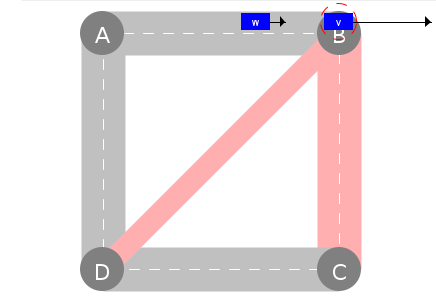
\includegraphics[scale=0.35]{../../events/vehicle-at-intersection-before.png}
		\caption{Vehicle arrives at segment end.}
		\label{fig:vehicle-at-intersection-before}
	\end{subfigure}
	\begin{subfigure}{.45\textwidth}
		\centering
		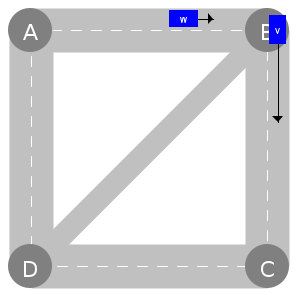
\includegraphics[scale=0.35]{../../events/vehicle-at-intersection-after.png}
		\caption{Vehicle arrives at segment start.}
		\label{fig:vehicle-at-intersection-after}
	\end{subfigure}
	\caption{Routing events.}
		\label{fig:routing-events}
\end{figure}

\noindent
\textbf{Vehicle arrives at segment end} (see Figure \ref{fig:vehicle-at-intersection-before})
occurs at time $t \in T$ if and only if there exists a vehicle $v \in V$ and a location $(s,d) \in L$ with segment $s \in S$ and traveled distance $d \in \mathbb{R}_0^+$ such that the vehicle $v$ at time $t$ is at location $(s,d)$, i.e. $S_{V.CL}(v,t) = (s,d)$, and the traveled distance $d$ on segment $s$ equals the length of the segment $s$, i.e. $P_{S.L}(s) = d$.

\vspace{4mm}
\noindent
\textbf{Vehicle arrives at segment start} (see Figure \ref{fig:vehicle-at-intersection-after})
occurs at time $t \in T$ if and only if there exists a vehicle $v \in V$ and a location $(s,d) \in L$ with segment $s \in S$ and traveled distance $d \in \mathbb{R}_0^+$ such that the vehicle $v$ at time $t$ is at location $(s,d)$, i.e. $S_{V.CL}(v,t) = (s,d)$, and the traveled distance $d$ on segment $s$ is zero, i.e. $d = 0$. Note that the event vehicle arrives at segment start occurs concurrenly with event vehicle arrives at segment end.
\vspace{-2mm}

\subsection{Driving and Overtaking Events}
\label{sec:overtaking-events}

This Section subsequently describes driving and overtaking events which occur between multiple vehicles, where former are visualized in Figure \ref{fig:overtaking-events}.

\begin{figure}
	\centering
	\begin{subfigure}{.45\textwidth}
	\centering
	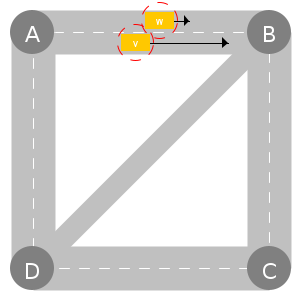
\includegraphics[scale=0.35]{../../events/faster-vehicle-front-at-slower-vehicle-back.png}
	\caption{Faster vehicle f.\ at slower vehicle b.}
	\label{fig:faster-vehicle-front-at-slower-vehicle-back}
	\end{subfigure}
	\begin{subfigure}{.45\textwidth}
	\centering
	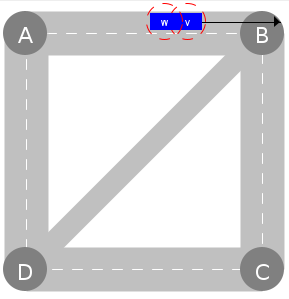
\includegraphics[scale=0.35]{../../events/slower-vehicle-front-at-faster-vehicle-back.png}
	\caption{Slower vehicle f.\ at faster vehicle b.}
	\label{fig:slower-vehicle-front-at-faster-vehicle-back}
	\end{subfigure}
	\caption{Overtaking events.}
	\label{fig:overtaking-events}
\end{figure}

\noindent
\textbf{Vehicle drive speed changes}
occurs at time $t \in T$ if and only if there exists a vehicle $v \in V$ with current drive speed $S_{V.CDS}(v, t)$, such that for all previous times $t' \in T$ with $t' < t$, where the current drive speed $S_{V.CDS}(v,t')$ of vehicle $v$ at time $t'$ was identical, i.e. $S_{V.CDS}(v,t') = S_{V.CDS}(v,t)$, there exists an intermediate time $t'' \in T$ with $t' < t'' < t$, such that the current drive speed $S_{V.CDS}(v,t'')$ of vehicle $v$ at time $t''$ is different, i.e. $S_{V.CDS}(v,t'') \neq S_{V.CDS}(v,t)$.
\vspace{4mm}

\noindent
\textbf{Faster vehicle front at slower vehicle back} (see Figure \ref{fig:faster-vehicle-front-at-slower-vehicle-back})
occurs at time $t \in T$ if and only if there exists a faster vehicle $v_{f} \in V$ as well as a slower vehicle $v_{s} \in V$, such that 
\begin{enumerate}
\item the current drive speed of the faster vehicle $v_{f}$ at time $t$ is greater than the current drive speed of the slower vehicle $v_{s}$, i.e. $ S_{V.CDS}(v_{f},t) > S_{V.CDS}(v_{s},t)$, and
\item the locations of the vehicles at time $t$, i.e. $S_{V.CL}(v_{f},t) = (s_{vf}, d_{vf})$ and  $S_{V.CL}(v_{s},t) = (s_{vs}, d_{vs})$ are such that the segments $s_{vf}, s_{vs}$ of both faster and slower vehicle match, and the travelled distance of the faster vehicle plus the faster vehicles half-length equals the travelled distance of the slower vehicle minus the slower vehicles half-length, i.e. $d_{vf} + \frac{P_{V.L}(v_{vf})}{2} = d_{vs} - \frac{P_{V.L}(v_{vs})}{2}$.
\end{enumerate}
\vspace{4mm}

\noindent
\textbf{Slower vehicle front at faster vehicle back} (see Figure \ref{fig:slower-vehicle-front-at-faster-vehicle-back})
occurs at time $t \in T$ if and only if there exists a faster vehicle $v_{f} \in V$ as well as a slower vehicle $v_{s} \in V$, such that 
\begin{enumerate}
	\item the current drive speed of the faster vehicle $v_{f}$ at time $t$ is greater than the current drive speed of the slower vehicle $v_{s}$, i.e. $ S_{V.CDS}(v_{f},t) > S_{V.CDS}(v_{s},t)$, and
	\item the locations of the vehicles at time $t$, i.e. $S_{V.CL}(v_{f},t) = (s_{vf}, d_{vf})$ and  $S_{V.CL}(v_{s},t) = (s_{vs}, d_{vs})$ are such that the segments $s_{vf}, s_{vs}$ of both faster and slower vehicle match, and the travelled distance of the faster vehicle minus the faster vehicles half-length equals the travelled distance of the slower vehicle plus the slower vehicles half-length, i.e. $d_{vf} - \frac{P_{V.L}(v_{vf})}{2} = d_{vs} + \frac{P_{V.L}(v_{vs})}{2}$.
\end{enumerate}
\vspace{-2mm}

\subsection{Demand Events}
\label{sec:demand-events}
This Section describes demand events which occur based on demand appearance or vehicle positioning at demand pick-up or demand drop-off locations, which are visualized in Figure \ref{fig:demand-events}, and which we describe subsequently.

\begin{figure}
	\begin{subfigure}{.32\textwidth}
		\centering
		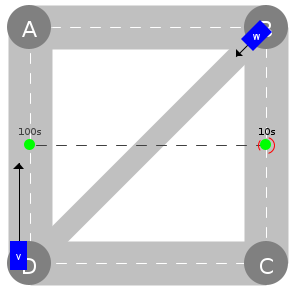
\includegraphics[scale=0.35]{../../events/demand.png}
		\caption{Demand appears.}
		\label{fig:demand-appears}
	\end{subfigure}
	\hfill
	\begin{subfigure}{.32\textwidth}
		\centering
		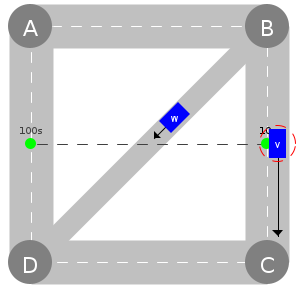
\includegraphics[scale=0.35]{../../events/vehicle-at-demand-pick-up.png}
		\caption{Vehicle at demand pick-up.}
		\label{fig:vehicle-at-demand-pick-up}
	\end{subfigure}
	\hfill
	\begin{subfigure}{.32\textwidth}
		\centering
		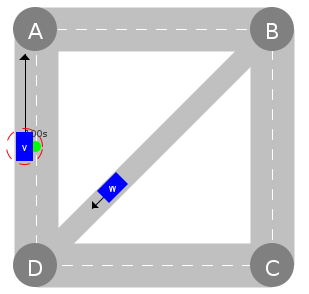
\includegraphics[scale=0.35]{../../events/vehicle-at-demand-drop-off.png}
		\caption{Vehicle at demand drop-off.}
		\label{fig:vehicle-at-demand-drop-off}
	\end{subfigure}
\hfill
	\caption{Demand events.}
	\label{fig:demand-events}	
\end{figure}

\noindent
\textbf{Demand appears} (see Figure \ref{fig:demand-appears}) 
occurs at time $t \in T$ if and only if there exists a vehicle $v \in V$ and a demand $d \in D$, such that the demand $d$ at time $t$ doesn't have an assigned current vehicle $v$, i.e. $S_{D.CV}(d, t) = \{\perp\}$, and such that the demands appear time $P_{D.AT}$ equals the current time $t$, i.e. $P_{D.AT} = t$.

\vspace{4mm}

\noindent
\textbf{Vehicle arrives at demand pick-up location} (see Figure \ref{fig:vehicle-at-demand-pick-up}) 
occurs at time $t \in T$ if and only if there exists a vehicle $v \in V$ and a demand $d \in D$ with demand pick-up location $l_d^{PULT}$, such that the vehicle $v$ at time $t$ is at demand pick-up location, i.e. $S_{V.CL}(v, t) = l_d^{PULT}$, and for all previous times $t' \in T$ with $t' < t$ where vehicle $v$ was at location $l_d^{PULT}$, i.e. $S_{V.CL}(v, t') = l_d^{PULT}$, there exists an intermediate time $t'' \in T$ with $t' < t'' < t$, such that vehicle $v$ was not at location $l_d^{PULT}$, i.e. $S_{V.CL}(v, t'') \neq l_d^{PULT}$.

\vspace{4mm}

\noindent
\textbf{Vehicle arrives at demand drop-off location} (see Figure \ref{fig:vehicle-at-demand-drop-off})
occurs at time $t \in T$ if and only if there exists a vehicle $v \in V$ and a demand $d \in D$ with demand drop-off location $l_d^{DOLT}$, such that the vehicle $v$ at time $t$ is at demand drop-off location, i.e. $S_{V.CL}(v, t) = l_d^{DOLT}$, and for all previous times $t' \in T$ with $t' < t$ where vehicle $v$ was at location $l_d^{DOLT}$, i.e. $S_{V.CL}(v, t') = l_d^{DOLT}$, there exists an intermediate time $t'' \in T$ with $t' < t'' < t$, such that vehicle $v$ was not at location $l_d^{DOLT}$, i.e. $S_{V.CL}(v, t'') \neq l_d^{DOLT}$.

\vspace{-2mm}

\subsection{Charging Events}
This Section subsequently describes charging events which occur based on vehicle positioning at charging stations or based on their charge speed. 

\vspace{4mm}

\label{sec:charging-events}
\noindent
\textbf{Vehicle arrives at charging station}
occurs at time $t \in T$ if and only if there exists a vehicle $v \in V$ and a charging station $cs \in CS$ with location $l = P_{CS.L}(cs)$, such that the vehicle $v$ at time $t$ is at location $l$, i.e. $S_{V.CL}(v, t) = l$, and for all previous times $t' \in T$ with $t' < t$ where vehicle $v$ was at location $l$, i.e. $S_{V.CL}(v, t') = l$, there exists an intermediate time $t'' \in T$ with $t' < t'' < t$, such that vehicle $v$ was not at location $l$, i.e. $S_{V.CL}(v, t'') \neq l$.

%\vspace{4mm}
%\noindent
%\textbf{Vehicle starts charging}
%occurs at time $t \in T$ if and only if there exists a vehicle $v \in V$ such that the current charge speed of vehicle $v$ at time $t$ is not zero, i.e. $S_{V.CCS}(v,t) \neq 0$, and for all previous times $t' \in T$ with $t' < t$, where the current charge speed of vehicle $v$ is not zero, i.e. $S_{V.CCS}(v,t') \neq 0$, there exists an intermediate time $t'' \in T$ with $t' < t'' < t$, such that the current charge speed of vehicle $v$ is zero, i.e. $S_{V.CCS}(v,t'') = 0$.

\vspace{4mm}
\noindent
\textbf{Vehicle charge speed changes}
occurs at time $t \in T$ if and only if there exists a vehicle $v \in V$ with current charge speed $S_{V.CCS}(v, t)$, such that for all previous times $t' \in T$ with $t' < t$, where the current charge speed $S_{V.CCS}(v,t')$ of vehicle $v$ at time $t'$ was identical, i.e. $S_{V.CCS}(v,t') = S_{V.CCS}(v,t)$, there exists an intermediate time $t'' \in T$ with $t' < t'' < t$, such that the current charge speed $S_{V.CCS}(v,t'')$ of vehicle $v$ at time $t''$ is different, i.e. $S_{V.CCS}(v,t'') \neq S_{V.CCS}(v,t)$.

%\vspace{4mm}
%\noindent
%\textbf{Vehicle stops charging}
%occurs at time $t \in T$ if and only if there exists a vehicle $v \in V$ such that the current charge speed of vehicle $v$ at time $t$ is zero, i.e. $S_{V.CCS}(v,t) = 0$, and for all previous times $t' \in T$ with $t' < t$, where the current charge speed of vehicle $v$ is zero, i.e. $S_{V.CCS}(v,t') = 0$, there exists an intermediate time $t'' \in T$ with $t' < t'' < t$, such that the current charge speed of vehicle $v$ is not zero, i.e. $S_{V.CCS}(v,t'') \neq 0$.
\vspace{-2mm}

\noindent
\subsection{Battery Events}
\label{sec:battery-events}
This Section describes battery events which occur based on vehicle battery level. We describe these events subsequently.
\vspace{4mm}

\noindent
\textbf{Vehicle battery becomes empty}
occurs at time $t \in T$ if and only if there exists a vehicle $v \in V$ such that the current battery level of vehicle $v$ at time $t$ is zero, i.e. $S_{V.CBL}(v,t) = 0$ and for all previous times $t' \in T$ with $t' < t$, where the current battery level of vehicle $v$ was zero, i.e. $S_{V.CBL}(v,t') = 0$, there exists an intermediate time $t'' \in T$ with $t' < t'' < t$, such that the current battery level of vehicle $v$ was not zero, i.e. $S_{V.CBL}(v,t'') \neq 0$.

\vspace{4mm}
\noindent
\textbf{Vehicle battery becomes full}
occurs at time $t \in T$ if and only if there exists a vehicle $v \in V$ such that the current battery level of vehicle $v$ at time $t$ equals the maximum battery level of vehicle $v$, i.e. $S_{V.CBL}(v,t) = P_{V.MBL}(v)$, and for all previous times $t' \in T$ with $t' < t$, where the current battery level of vehicle $v$ equals the maximum battery level of vehicle $v$, i.e. $S_{V.CBL}(v,t') = P_{V.MBL}(v)$, there exists an intermediate time $t'' \in T$ with $t' < t'' < t$, such that the current battery level of vehicle $v$ does not equal the maximum battery level of vehicle $v$, i.e. $S_{V.CBL}(v,t'') \neq P_{V.MBL}(v)$.

% TODO Section Headings rework, e.g. charge speed, drive speed
%\subsection{Speed Events}
%Adapt existing section headings
\vspace{-2mm}

\section{Conclusion and Outlook}
\label{sec:con}
%we proposed a simulation environment for transportation system design, which is based on a formal system theory. For this, 
In this work, we presented a formalization of essential static properties, dynamic state functions, as well as events concisely describing transportation system design space in the scope of emerging transportation paradigms such as autonomous vehicles, demand-responsive transport and the transportation electrification. Our proposed formalization allows for reduction of simulation complexity by focusing on relevant events impacting the design problem at hand only, while omitting unimportant details negatively impacting simulation performance, thereby reducing both modeling as well as simulation effort. In addition, the provided formalization of system theory and discrete events serves as an interface for deriving well-defined system structure and efficient control strategies. Future work includes demonstration as well as approach application for deriving control strategies based on our proposed formalization.

%Future work
\vspace{-2mm}

\bibliographystyle{plain}
\bibliography{main}
\end{document}
